% (c) 2015 Daniele Zambelli daniele.zambelli@gmail.com

% % \vspace{-2ex}% (c) 2012 Dimitrios Vrettos - d.vrettos@gmail.com
  \begin{center}
    \begin{hieroglyph}{\leavevmode \loneSign{\Aca GM/43/}\HinterSignsSpace
\loneSign{\Aca GM/43/}\HinterSignsSpace
\loneSign{\Aca GM/43/}\HinterSignsSpace
\Cadrat{\CadratLineI{\Aca GV/32/\hfill\Aca GV/32/\hfill\Aca GV/32/}\CadratLine{\Aca GV/32/\hfill\Aca GV/32/\hfill\Aca GV/32/}}\HinterSignsSpace
\Cadrat{\CadratLineI{{\Hsmaller\Hsmaller\Aca GV/51/}\hfill{\Hsmaller\Hsmaller\Aca GV/51/}\hfill{\Hsmaller\Hsmaller\Aca GV/51/}}\CadratLine{\Aca GV/51/\hfill\Aca GV/51/\hfill\Aca GV/51/\hfill\Aca GV/51/}}\HinterSignsSpace
\loneSign{\Aca GZ/32/}\HinterSignsSpace
\loneSign{\Aca GZ/32/}\HinterSignsSpace
\loneSign{\Aca GZ/32/}}\end{hieroglyph}
  \end{center}\vspace{-2ex}
% \begin{inaccessibleblock}
% [Immagine di una porzione dell'insieme di Mandelbrot.]
% \vspace{-2ex}
% \begin{center} 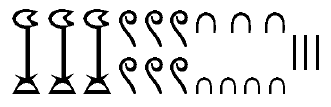
\includegraphics[scale=0.25]{img/hiero3673.png} \end{center}
% \vspace{-2ex}
% \end{inaccessibleblock}

% (c) 2014 Daniele Zambelli - daniele.zambelli@gmail.com
% 
% Tutti i grafici per il capitolo relativo alle parabole
%
% 

\newcommand{\espdueterzi}{% 
    % Esponenziali con basi diverse.
    \disegno{
    \rcom{-10}{+10}{-1}{10}{gray!50, very thin, step=1}
    \begin{scope}[ultra thick, color=Maroon!50!black]
     \tkzInit[xmin=-10.3, xmax=+10.3, ymin=-0.3, ymax=+10.3]
     \tkzFct[domain=-10.3:+6]{(3./2)**x}
     \tkzFct[color=Green!50!black, domain=-6:+10.3]{(2./3)**x}
     \begin{scope}[color=Black!50!black]
      \filldraw (1, 3./2) circle (1.2pt);
      \filldraw (1, 2./3) circle (1.2pt);
     \end{scope}
     \filldraw [color=Red](0, 1) circle (1.2pt);  
    \end{scope}
    \begin{scope}[color=black]
     \draw (-7.3, 7) node{\(f(x)=\tonda{\dfrac{2}{3}}^x\)}; 
     \draw ((7.3, 7) node{\(f(x)=\tonda{\dfrac{3}{2}}^x\)};
    \end{scope}
    }
}

\newcommand{\logduebasi}{% 
    % Esponenziali con basi diverse.
    \disegno{
    \rcom{-1}{+10}{-9}{9}{gray!50, very thin, step=1}
    \begin{scope}[ultra thick, color=Maroon!50!black]
      \tkzInit[xmin=-1.3, xmax=+80, xstep=.5, ymin=-10.3,ymax=+10.3]
      \tkzFct[domain=.01:+10]{log(x)/log(2)}
      \filldraw (2, 1) circle (1.2pt);
      \begin{scope}[color=Green!50!black]
        \tkzFct[domain=-.01:+10]{log(x)/log(1./2)}
        \filldraw (2, -1) circle (1.2pt);
      \end{scope}
    \end{scope}
    \begin{scope}[color=black]
      \draw (9.5, 2.8) node{a=2}; 
      \draw (9.5, -2.8) node{a=0.5};
    \end{scope}
      \filldraw [color=Red] (1,0) circle (1.2pt);
    }
}


\chapter{Iperreali}
\label{sec:01_introduzione}
Lo scopo di questo capitolo è riprendere familiarità con l'uso 
dei numeri iperreali, già descritti verso la fine del terzo anno. 
Le parti principali utili ai fini della nostra trattazione sono 
direttamente riportate dal terzo volume.\\
Il motivo di questi richiami è che in analisi matematica è normale 
avere a che fare con quantità infinitesime e quantità infinite e 
valutare il comportamento delle funzioni applicate a tali quantità. 
Quindi l'uso dei numeri iperreali diviene vantaggioso.\\
La conoscenza degli iperreali non è molto diffusa neanche fra i matematici, 
abituati da un secolo e mezzo a procedimenti più impegnativi e sofisticati.
La ragione per la quale noi invece ne facciamo uso è che ci rendono il calcolo 
più semplice e immediato, senza per questo nuocere al rigore e alla 
precisione dei ragionamenti.

\section{Alcune questioni importanti sui numeri in $\R$}
\label{sec:insnum_reali}

I numeri reali formano un insieme \emph{ordinato}, \emph{denso} e 
\emph{completo}: $\R$. È un insieme ordinato perché fra due numeri reali
diversi sappiamo sempre indicare il maggiore e il minore. È denso
perché fra due numeri reali diversi, per quanto vicini, se ne può 
sempre trovare almeno un altro. E infine \(\R\) è un insieme completo 
perché il numero che troveremo fra i due vicini è ancora un numero reale.\\
Possiamo quindi far corrispondere ad ogni punto della \emph{retta reale} un 
numero \emph{reale} e, viceversa, ad ogni numero \emph{reale} un punto 
della \emph{retta reale}. In poche parole, siamo
autorizzati a pensare la retta reale come una retta ``priva di buchi'':
c'è almeno un punto
in ogni posizione, anche osservando la retta al microscopio, 
con qualsiasi ingrandimento (ingrandimento reale, come vedremo).\\
Se usiamo la retta reale come immagine dell'insieme \(\R\) è perché
si tratta di una rappresentazione efficace. Ma ricordiamoci sempre che un insieme 
in matematica è un oggetto astratto, quindi la retta reale è solo
un modello che ci aiuta a capire le proprietà dell'insieme \(\R\).\\
Per esempio, a proposito dell'ordinamento in \(\R\), ci riesce facile
posizionare i numeri sulla retta, in corripondenza di punti più vicini o più lontani 
dall'origine. Così possiamo verificare anche un'ulteriore proprietà, la 
\emph{proprietà archimedea}: per quanto piccolo sia un numero, si può 
sempre trovare una moltiplicazione tale che il prodotto superi altro numero
prefissato.
Sulla retta: dati due segmenti con un estremo nell'origine, potrai sempre moltiplicare
la lunghezza del più breve, in modo che diventi maggiore dell'altro.\\
A causa della completezza di \(\R\), non è possibile inserire
nella retta reale dei punti che non corrispondano a numeri reali. Se inseriamo numeri
di nuovo tipo, il modello cambia. Il nuovo insieme e la nuova retta sono
diversi dall'insieme dei reali e dalla retta reale: si perde qualche proprietà 
e se ne acquisiscono di nuove.
Infatti...

% \vspace{24pt}

\section{I numeri Iperreali e l'insieme $\IR$}
\label{sec:insnum_iperreali}

In questa sezione vedremo un nuovo insieme di numeri, utile a modellizzare e 
risolvere nuove classi di problemi. Rispetto a quanto già sappiamo dell'insieme 
\(\R\), dovremo adattare alcune regole di calcolo e riscontreremo proprietà nuove, mentre 
dovremo abbandonarne una delle più note e utili. 

\subsection{Il problema della velocità}
\label{subsec:insnum_velocita}

Alla fine del 1600 Newton e Leibniz studiavano problemi legati alla meccanica. 
Una delle grandezze alla base della meccanica è la \emph{velocità}. Ma cosa è 
la velocità? Se l'oggetto A percorre più strada dell'oggetto B possiamo dire 
che A è più veloce di B? No, non basta misurare lo spazio percorso da un 
oggetto per calcolare la sua velocità, bisogna anche misurare il tempo 
impiegato a percorrere quello spazio. Infatti sappiamo che dire che:
\[velocità = \frac{spazio percorso}{tempo impiegato}\]

La grandezza calcolata in questo modo è \emph{la velocità media} dell'oggetto, 
ma in ogni istante del percorso l'oggetto ha una propria velocità. 
Un modo molto pratico di ottenere la velocità media è di tenere conto 
del percorso totale e dividerlo per il tempo complessivo impiegato a percorrerlo.
Insomma, se ho percorso in bicicletta  \(8\) chilometri in mezz'ora, la mia media è 
di  \(16 km/h\). Nel percorso avrò rallentato in salita, accelerato in discesa, 
mi sarò fermato agli stop e ai semafori, ecc., e la mia velocità media si ottiene
dalla media delle velocità che ho realizzato istante per istante.\\
Posso sapere la velocità di ogni istante? Potrei misurare gli spazi percorsi in  
intervalli di tempo molto piccoli, così calcolerei le velocità relative a tratti 
molto brevi. Ma sarebbero sempre velocità medie. Più 
restringo l'intervallo di tempo, più la velocità media si avvicina alla 
velocità istantanea \dots ma resta sempre una velocità media.

Per trovare la velocità istantanea dovrei riuscire a isolare l'istante di tempo:
un numero (positivo) che rappresenta il tempo, più piccolo di qualunque altro numero.
L'unico numero reale positivo, più piccolo di qualunque numero, è lo zero, ma non posso
usarlo per il calcolo della velocità, perché la divisione per 
zero non è definita: i numeri reali non ci permettono di calcolare una 
grandezza così semplice e evidente come la velocità di un oggetto in un dato 
istante.

Servirebbe un insieme numerico con numeri positivi più piccoli di un 
qualsiasi altro numero positivo, ma diversi da zero! Ma è possibile 
trovare tali numeri nell'insieme dei reali che, come abbiamo visto, 
è un insieme (già) completo?



\subsection{Un nuovo insieme: gli Iperreali}
\label{subsec:insnum_iperreali}

All'insieme dei numeri reali aggiungiamo un nuovo numero (non reale):

\[\varepsilon > 0 \text{ tale che } 
\varepsilon < \frac{1}{n} \text{ per qualunque } n \in \N\]

tradotto in simboli:

\[\varepsilon > 0 \quad | \quad \varepsilon < \frac{1}{n} \quad \forall n \in 
\N\]

Un numero siffatto lo chiameremo un \emph{infinitesimo} e lo indicheremo 
con una lettera minuscola dell'alfabeto greco, per esempio $\epsilon$.
Per quanto è già stato detto, un tale numero non può essere un numero
reale. 

La prima conseguenza all'introduzione di un infinitesimo è che allora ce ne 
sono infiniti! Infatti anche la metà di un infinitesimo è un infinitesimo e 
anche il suo doppio o un suo sottomultiplo o un suo multiplo. (Per verificarlo,
vedi le tabelle successive; per le conseguenze, vedi il paragrafo 10.) 

Altra conseguenza dell'aggiunta di un elemento infinitesimo all'insieme dei 
reali è che se esiste un numero maggiore di zero più piccolo di tutti gli altri 
numeri allora esiste anche un numero maggiore di qualunque altro numero:

\[\text{se} \quad \varepsilon < \frac{1}{n} \quad \forall n \in \N 
\quad \text{allora} \quad \frac{1}{\varepsilon} > n \quad \forall n 
\in \N\]

Quindi se aggiungiamo all'insieme dei reali un numero infinitesimo e possiamo 
usarlo nelle usuali 4 operazioni, allora in quell'insieme avremo un 
numero infinito di infinitesimi e un numero infinito di infiniti.

Chiamiamo \emph{iperreali} l'insieme numerico così ottenuto e lo indichiamo con 
il simbolo:~$\IR$.

\subsection{Tipi di Iperreali}
\label{subsec:insnum_iperreali}

Abbiamo visto che l'introduzione di un elemento nuovo, così piccolo
da poterlo pensare trascurabile, ha 
reso piuttosto affollato il nuovo insieme numerico. Cerchiamo di fare un po' 
di ordine. L'insieme degli Iperreali contiene:

\begin{itemize} [noitemsep]
 \item i numeri reali che d'ora in poi verranno chiamati anche numeri 
\emph{standard}, tra questi c'è anche lo zero;
 \item gli infinitesimi, lo zero è l'unico infinitesimo che è anche un numero 
reale;
 \item i numeri non reali che non sono né infinitesimi né infiniti;
 \item gli infiniti, nessun infinito ha una corrispondenza con i numeri reali.
\end{itemize}

Possiamo vedere questo insieme anche come formato dai seguenti elementi:

\begin{description} [noitemsep]
 \item \textbf{zero}
 è un infinitesimo ed è un numero standard;
 \item \textbf{infinitesimi non nulli}
 tutti gli infinitesimi diversi da zero;
 \item \textbf{finiti}
 tutti quei numeri che sono, in valore assoluto, minori di un numero reale;
 \item \textbf{finiti non infinitesimi}
 tutti quei numeri che sono in valore assoluto compresi tra due numeri reali 
 diversi da zero;
 \item \textbf{infiniti}
 tutti quei numeri che sono maggiori di qualsiasi numero reale

\end{description}
 
Per semplificare la scrittura (e complicare la lettura) adotteremo delle sigle 
e delle convenzioni per indicare questi diversi tipi di numeri:

\begin{center}
\begin{tabular}{ccc}\toprule
tipo & sigla & simboli\\\midrule
zero &  & 0\\
infinitesimo & \emph{i} & \\
infinitesimo non nullo & \emph{inn} & $\alpha, \beta, \gamma, \delta, \dots$\\
finito non infinitesimo& \emph{fni} & a, b, c, d, ...\\
finito & \emph{f} & a, b, c, d, ...\\
infinito & \emph{I} & A, B, C\\
qualsiasi &  & x, y, z, \ldots\\\bottomrule
\end{tabular}
\label{tab:insnum_tipi}
\end{center}

\subsection{Iperreali finiti e parte standard}
\label{subsec:insnum_partestandard}

Gli Iperreali finiti sono quei numeri che sono compresi tra due numeri Reali:

\begin{definizione}
 Il numero Iperreale $x$ è compreso tra due numeri Reali allora $x$ è un 
Iperreale finito:

\[\text{Se } x \in \IR \wedge a, b \in \R \wedge 
  a < x < b \text{ allora } x \text{ è un Iperreale finito.}\]
\end{definizione}

Ogni numero finito può essere visto come la somma di un numero reale più un 
Infinitesimo: se $x$ è finito allora $x = a + \epsilon$, quindi 
$x=a+\epsilon\approx a$. Si può immaginare ogni Iperreale finito come una
nuvola contenente un numero standard $a$ e tutti gli infinitesimi che lo 
circondano, così vicini ad $a$ da non potersi confondere con altri infiniti
infinitesimi di una nuvola vicina, appartenenti per esempio al numero Iperreale
$y=b+\epsilon$. Un numero Iperreale finito non può essere infinitamente vicino 
a due numeri reali diversi quindi esiste un solo numero Reale infinitamente 
vicino ad un numero Iperreale. 
Questo numero reale si chiama \emph{parte standard} del numeri Iperreale.

\begin{definizione}
 La parte standard di un numero Iperreale finito è il l'unico numero Reale 
infinitamente vicino:

\[\text{Se } x \in \IR \wedge x= a+\epsilon \text{ allora } 
a= \st(x) \text{ (st = parte standard).}\]
\end{definizione}


\subsection{Retta Iperreale e strumenti ottici}
\label{subsec:insnum_retta}

In un paragrafo precedente abbiamo visto che si può accettare il postulato che 
dice che ad ogni numero reale corrisponde un punto della retta e ad ogni 
punto della retta corrisponde un numero reale. 
Questa affermazione non è un teorema dimostrato, è un postulato. Fa parte del modello
di numeri usato, cioè è caratteristico dei numeri reali. Giacché ora stiamo cambiando
modello, cambiamo anche questo postulato. Lo riformuliamo così:

\begin{postulato}
Ad ogni numero Iperreale corrisponde un punto della retta (iperreale) e ad ogni 
punto della retta (iperreale) corrisponde un numero Iperreale.
\end{postulato}

Oppure:

\begin{postulato}
C'è una corrispondenza biunivoca tra i numeri Iperreali e 
i punti della retta (iperreale).
\end{postulato}

Con i numeri reali abbiamo una certa abitudine a rappresentare numeri.
Per rappresentare i numeri Iperreali dobbiamo procurarci degli strumenti 
particolari: \emph{microscopi}, \emph{telescopi}, \emph{grandangoli}.

Diamo una sbirciata al loro manuale di istruzioni.

\subsubsection{Microscopi}
\label{subsec:insnum_microscopio}

Il microscopio permette di ingrandire una porzione di retta. 
Un microscopio permette di visualizzare i seguenti numeri:

\begin{multicols}{4}
\begin{itemize}
 \item $+5,004$
 \item $-3,000002$
 \item $2-\epsilon$
 \item $-4+\delta$
\end{itemize}
\end{multicols}

Si può osservare come ci siano microscopi ``standard'' che ingrandiscono un 
numero \emph{naturale} di volte e microscopi ``non standard'' che ingrandiscono 
infinite volte.

\subsubsection{Telescopi}
\label{subsec:insnum_microscopio}

Il telescopio permette di avvicinare una porzione di retta senza cambiare la 
sua scala. 
Con un telescopio possiamo visualizzare i seguenti numeri:

\begin{multicols}{4}
\begin{itemize}
 \item $+127034$
 \item $-3600$
 \item $A+3$
 \item $-B+2$
\end{itemize}
\end{multicols}

Anche per i telescopi, i modelli più moderni offrono la possibilità di operare 
ingrandimenti ``standard'' o ``non standard'' a piacere.

\subsubsection{Grandangoli (Zoom)}
\label{subsec:insnum_microscopio}

Il Grandangolo permette di cambiare la scala della visualizzazione della retta, 
in questo modo possiamo far rientrare nel campo visivo anche numeri molto 
lontani.
Possiamo usare uno zoom per visualizzare i seguenti numeri:

\begin{multicols}{4}
\begin{itemize}
 \item $500$
 \item $-3000$
 \item $2A$
 \item $3B$
\end{itemize}
\end{multicols}

Anche per questi strumenti utilizzeremo versioni che permettono zoomate 
``standard'' e ``non standard''.

\subsection{Operazioni}
\label{subsec:insnum_operazioni}

Vediamo di seguito alcune regole relative alle operazioni 
che valgono nei numeri Iperreali.

\subsubsection{Addizione}
\label{subsec:insnum_addizione}

Alcune osservazioni:
\begin{enumerate} [noitemsep]
 \item Le regole relative all'addizione valgono anche per la sottrazione, se 
uno degli addendi è negativo. 
 \item Zero è l'elemento neutro dell'addizione nei Reali e continua ad esserlo 
anche negli Iperreali: $x+0=0+x=x$.
 \item Un infinitesimo più un altro infinitesimo dà per risultato un 
infinitesimo: $\alpha+\beta=\gamma$.
 \item Un infinitesimo non nullo più un altro infinitesimo non nullo può dare 
per risultato anche zero: \dots
 \item Un finito più un infinitesimo dà come risultato un finito.
 \item Un finito più un finito dà come risultato un finito.
 \item Un finito più un finito può dare come risultato un infinitesimo.
%  \item Un infinito più un infinitesimo dà come risultato un infinito.
 \item Un infinito più un finito dà come risultato un infinito.
 \item Un infinito più un infinito può dare come risultato zero, un 
infinitesimo, un finito non infinitesimo, un finito, un infinito.
\end{enumerate}

Nel precedente elenco abbiamo visto che alcune addizioni danno un risultato 
che dipende solo dai tipi degli operandi, altre operazioni danno dei risultati 
che dipendono dal valore degli operandi. Possiamo costruire una tabella che 
organizza le precedenti osservazioni.

\begin{center}
\renewcommand{\arraystretch}{.0}
\scalebox{0.8}{
\begin{tabular}{p{.7cm}|p{.7cm}|p{.7cm}|p{.7cm}|p{.7cm}|p{.7cm}|}
\centra{$+$} & \centra{0} & \centra{inn} & \centra{fni} & \centra{I} \\\hline
\centra{0} & \centra{0} & \centra{inn}& \centra{fni} & \centra{I} \\\hline
\centra{inn} & \centra{inn} & \centra{i}& \centra{fni} & \centra{I} \\\hline
\centra{fni} & \centra{fni} & \centra{fni}& \centra{f} & \centra{I} \\\hline
\centra{I} & \centra{I} & \centra{I}& \centra{I} & \centra{?} \\\hline
\end{tabular}}
\end{center}

\subsubsection{Moltiplicazione}
\label{subsec:insnum_moltiplicazione}

\noindent \begin{minipage}{.5\textwidth}
Alcune osservazioni:
\begin{enumerate} [noitemsep]
 \item Zero è l'elemento assorbente: il prodotto di un iperreale per zero
dà come risultato zero: $x \cdot 0=0 \cdot x=0$.
 \item Uno è l'elemento neutro della moltiplicazione nei Reali e continua ad 
esserlo anche negli Iperreali: $x \cdot 1=1 \cdot x=x$.
 \item Un infinitesimo per un altro infinitesimo dà per risultato un 
infinitesimo: $\alpha \cdot \beta=\gamma$.
 \item Un infinitesimo non nullo per un altro infinitesimo non nullo dà 
per risultato un infinitesimo non nullo.
 \item \dots
 \item \dots
 \item Il prodotto fra un finito e un infinitesimo apre a importanti riflessioni
sulla proprietà archimedea. Ne parliamo più avanti, in un paragrafo dedicato.
 \end{enumerate}
\end{minipage}
\hfill
\begin{minipage}{.45\textwidth}
E la tabella corrispondente:
\begin{center}
\renewcommand{\arraystretch}{.0}
\scalebox{0.8}{
\begin{tabular}{p{.7cm}|p{.7cm}|p{.7cm}|p{.7cm}|p{.7cm}|p{.7cm}|}
\centra{$\times$} & \centra{0} & \centra{1} & 
\centra{inn} & \centra{fni} & \centra{I} \\\hline
\centra{0} & \centra{0} & \centra{0} & 
\centra{0}& \centra{0} & \centra{0} \\\hline
\centra{1} & \centra{0} & \centra{1} & 
\centra{inn} & \centra{fni} & \centra{I} \\\hline
\centra{inn} & \centra{0} & \centra{inn} & 
\centra{inn}& \centra{inn} & \centra{?} \\\hline
\centra{fni} & \centra{0} & \centra{fni} & 
\centra{inn}& \centra{fni} & \centra{I} \\\hline
\centra{I} & \centra{0} & \centra{I} & 
\centra{?}& \centra{I} & \centra{I} \\\hline
\end{tabular}}
\end{center}
\vspace{2mm}
\end{minipage}

\subsubsection{Divisione}
\label{subsec:insnum_divisione}


\noindent \begin{minipage}{.5\textwidth}
Alcune osservazioni:
\begin{enumerate} [noitemsep]
 \item Anche negli Iperreali la divisione per zero non è definita.
 \item Uno può essere visto come un elemento neutro solo destro: $x \div 1=x$.
 \item Per cercare i risultati possiamo rifarci alla definizione di quoziente.
 \item \dots
%  \item Un infinitesimo per un altro infinitesimo dà per risultato un 
% infinitesimo: $\alpha \cdot \beta=\gamma$.
%  \item Un infinitesimo non nullo per un altro infinitesimo non nullo da 
% per risultato un infinitesimo non nullo.
%  \item Un finito per un infinitesimo dà come risultato un finito.
%  \item Un finito per un finito dà come risultato un finito.
%  \item Un finito per un finito può dare come risultato un infinitesimo.
% %  \item Un infinito per un infinitesimo dà come risultato un infinito.
%  \item Un infinito per un finito dà come risultato un infinito.
%  \item Un infinito per un infinito può dare come risultato zero, un 
% infinitesimo, un finito non infinitesimo, un finito, un infinito;
\end{enumerate}
\vspace{20mm}
\end{minipage}
\hfill
\begin{minipage}{.45\textwidth}
E la tabella corrispondente:
\begin{center}
\renewcommand{\arraystretch}{.0}
\scalebox{0.8}{
\begin{tabular}{p{.7cm}|p{.7cm}|p{.7cm}|p{.7cm}|p{.7cm}|p{.7cm}|}
% \begin{tabular}{c|c|c|c|c|c|}
\centra{$\div$} & \centra{0} & \centra{1} & 
\centra{inn} & \centra{fni} & \centra{I} \\\hline
\centra{0} &  & \centra{0} & 
\centra{0}& \centra{0} & \centra{0} \\\hline
\centra{1} &  & \centra{1} & 
\centra{I} & \centra{fni} & \centra{inn} \\\hline
\centra{inn} &  & \centra{inn} & 
\centra{?}& \centra{inn} & \centra{inn} \\\hline
\centra{fni} &  & \centra{fni} & 
\centra{I}& \centra{fni} & \centra{inn} \\\hline
\centra{I} &  & \centra{I} & 
\centra{I}& \centra{I} & \centra{?} \\\hline
\end{tabular}}
\end{center}
\end{minipage}

\subsubsection{Reciproco}
\label{subsec:insnum_reciproco}

\noindent \begin{minipage}{.5\textwidth}
Alcune osservazioni:
\begin{enumerate} [noitemsep]
 \item Dalla tabella precedente si può estrarre la riga corrispondente a~1
e si ottiene la tabella del reciproco.
 \item Una volta convinti della regola del reciproco, si può ricavare la 
tabella della divisione attraverso la 
regola:~$x \div y = x \times \tonda{\frac{1}{y}}$.
\end{enumerate}
\end{minipage}
\hfill
\begin{minipage}{.45\textwidth}
E la tabella corrispondente:
\begin{center}
\renewcommand{\arraystretch}{.0}
\scalebox{0.8}{
\begin{tabular}{p{1.7cm}|p{.7cm}|p{.7cm}|p{.7cm}|p{.7cm}|p{.7cm}|}
\centra{numero} & \centra{0} & \centra{1} & 
\centra{inn} & \centra{fni} & \centra{I} \\\hline
\centra{reciproco} &  & \centra{1} & 
\centra{I} & \centra{fni} & \centra{inn} %\\\hline
\end{tabular}}
\end{center}
\vspace{11mm}
\end{minipage}

\begin{osservazione}
Non ci sono regole immediate per le seguenti operazioni:
\begin{multicols}{4}
\begin{itemize} [nosep]
 \item \(\dfrac{\epsilon}{\delta}\)
 \item \(\dfrac{A}{B}\)
 \item \(A \cdot \epsilon\)
 \item \(A + B\)
\end{itemize}
\end{multicols}
In questi casi il tipo di risultato dipende dall'effettivo valore degli 
operandi. Ad esempio, nel caso del quoziente tra due infinitesimi possiamo 
trovarci nelle seguenti situazioni:
\begin{multicols}{3}
\begin{itemize} [nosep]
 \item \(\dfrac{\epsilon^2}{\epsilon} = \epsilon\) \quad (i)
 \item \(\dfrac{2\epsilon}{\epsilon} = 2\) \quad (fni)
 \item \(\dfrac{\epsilon}{\epsilon^2} = \frac{1}{\epsilon}\) \quad (I)
\end{itemize}
\end{multicols}
\end{osservazione}

Possiamo ora esercitarci nel calcolo con questi nuovi numeri. 
Continuiamo ad utilizzare la convenzione di indicare gli 
infinitesimi con lettere greche minuscole
($\alpha,~\beta,~\gamma,~\delta,~\epsilon,~\dots$), 
i finiti non infinitesimi con lettere latine minuscole 
($a,~b,~c~,~\dots,~m,~n,~\dots$) 
e gli infiniti con lettere latine maiuscole 
($A,~B,~C~,~\dots,~M,~N,~\dots$).

\begin{exrig}
Semplifichiamo le seguenti espressioni scrivendo il tipo di risultato ottenuto.

 \begin{esempio}
  $3\epsilon +5 +6M -2\epsilon +7 -2M = 4M +12 +\epsilon \quad (tipo=I)$
 \end{esempio}

\begin{osservazione}
Quando il risultato è la somma di più elementi, li scriviamo, ordinandoli dal 
più grande, in valore assoluto, al più piccolo.
%  Quando possibile scriviamo un risultato composto da più elementi scrivendoli 
% dal più grande, in valore assoluto, al più piccolo.
\end{osservazione}

 \begin{esempio}
\(7 +8M -5\epsilon  -4 +3\epsilon-2N = 8M -2N +3 -2\epsilon\)
\quad (tipo non definito)
 \end{esempio}
 
 \begin{esempio}
\(\tonda{3M +2\epsilon} \tonda{3M -2\epsilon} = 9M -4\epsilon\)
\quad (tipo=I)
 \end{esempio}
 
 \begin{esempio}
\(\tonda{M +3} \tonda{M -3} - \tonda{M+2}^2 +4\tonda{M +3}=\)

\(=M^2 -9 -M^2 -4M -4 +4M +12 = -1\)
\quad (tipo=fni)
 \end{esempio}
 
 \begin{esempio}
\(10a -\tonda{A +1}^2 -3a +2\tonda{a+2\alpha} +A^2 +6\tonda{b -3\alpha} +2A= \)

\(=10a -A^2 -2A -1 -3a +2a+4\alpha +A^2 +6b -18\alpha +2A = 9a +6b -14\alpha\) 
\quad (tipo=fni)
 \end{esempio}
\end{exrig}

% \subsection{Espressioni}
% \label{subsec:insnum_espressioni}

\subsection{Confronto}
\label{subsec:insnum_confronto}

L'insieme dei numeri Reali ha un ordinamento completo, se $a$ e $b$ sono due 
numeri reali qualunque è sempre valida una e una sola delle seguenti 
affermazioni:

\[a<b \quad a=b \quad b<a\]

Per confrontare due numeri Reali possiamo utilizzare le seguenti regole:

\begin{itemize} [noitemsep]
 \item qualunque numero negativo è minore di qualunque numero positivo;
 \item se due numeri sono negativi, è minore quello che ha il modulo maggiore;
 \item se $a$ e $b$ sono due numeri positivi, 
 $a<b \Leftrightarrow \frac{a}{b}<1 \text{ (o } a-b<0 \text{)}$.
\end{itemize}

Anche negli Iperreali valgono le proprietà dei Reali richiamate sopra. 
Ma l'insieme degli Iperreali non ha un ordinamento completo:
se di $\epsilon$ e $\delta$ sappiamo solo che sono due infinitesimi,
non è possibile dire se $\epsilon < \delta$ o $\epsilon > \delta$.
E questo si ripercuote anche su tutti gli altri numeri: senza ulteriori 
informazioni non possiamo dire se $a+\epsilon$ è maggiore minore o uguale 
a $a+\delta$. 
Problemi analoghi si incontrano nel confronto degli infiniti.
Vediamo allora come è possibile affrontare il problema del confronto tra 
Iperreali.

\begin{osservazione}
Manteniamo valide le regole per il confronto di numeri con segno diverso o numeri 
negativi. Possiamo quindi concentrare l'attenzione sul confronto dei soli numeri positivi.
Nei prossimi paragrafi assumeremo che le variabili si riferiscano solo a numeri 
positivi.
\end{osservazione}

Restringendo l'osservazione ai numeri positivi, possiamo affermare che:

Gli infinitesimi sono più piccoli dei non 
infinitesimi e i finiti sono più piccoli degli infiniti:

\[i \quad < \quad fni \quad < \quad I\]

Passiamo ora al confronto all'interno dei diversi tipi di numeri Iperreali.

\subsubsection{Confronto tra finiti non infinitesimi}
\label{subsubsec:insnum_confrontoreali}

Se due numeri Iperreali hanno parte standard diversa allora è maggiore quello 
che ha la parte standard maggiore:

\[x < y \Leftrightarrow \st(x) < st(y)\]

Nel caso i due numeri abbiano la stessa parte standard si deve studiare 
l'ordinamento degli infinitesimi, cosa che faremo nel prossimo paragrafo.

\subsubsection{Confronto tra infinitesimi}
\label{subsubsec:insnum_confrontoreali}

\begin{enumerate}
 \item Zero è minore di qualunque infinitesimo.\\
  Se sappiamo soltanto che $\epsilon$ e $\delta$ sono due infinitesimi 
  non possiamo stabilire quale dei due sia il maggiore e quale il minore. 
  Servono più informazioni. Vediamo alcuni esempi.

  \begin{esempio}
   Nel caso $\delta = \epsilon + \gamma$ con $\gamma$ infinitesimo positivo, 
   dato che~$\delta-\epsilon=\epsilon+\gamma-\epsilon=\gamma>0$, 
   $\delta$ sarà maggiore di $\epsilon$.
  \end{esempio}

  \begin{esempio}
   Nel caso $\delta = 2\epsilon$, 
   dato che~$\delta-\epsilon=2\epsilon-\epsilon=\epsilon>0$, 
   $\delta$ sarà maggiore di $\epsilon$.
  \end{esempio}

  \begin{esempio}
   Vediamo un altro modo per trattare il caso $\delta = 2\epsilon$, 
   dato che~$\frac{\delta}{\epsilon}=\frac{2\epsilon}{\epsilon}=2>1$, 
   $\delta$ sarà maggiore di $\epsilon$.
  \end{esempio}

  Questo secondo metodo permette di ricavare delle informazioni interessanti. 
  Vediamo alcuni esempi:

 \item Una parte infinitesima di un infinitesimo è più piccola di quell'infinitesimo.
  \begin{esempio}
   Se $\delta = \epsilon \cdot \gamma$, dato 
   che~$\frac{\delta}{\epsilon}=\frac{\epsilon \cdot \gamma}{\epsilon}=\gamma<1$, 
   $\delta$ sarà minore di $\epsilon$.
  \end{esempio}

  \begin{osservazione}
   In questo caso il rapporto non solo è più piccolo di~1 ma è addirittura un 
   \emph{infinitesimo}. 
   Quando il rapporto tra due infinitesimi è un infinitesimo 
   possiamo dire che il primo è un infinitesimo di \emph{ordine superiore} e si 
   scrive:~$\delta=o(\epsilon)$.
  \end{osservazione}

 \item Un infinitesimo è maggiore di una sua parte infinitesima.

  \begin{esempio}
   Se $\epsilon=\delta\cdot\gamma$, dato che 
   $\frac{1}{\epsilon}=\frac{1}{\delta\cdot \gamma}$, si ha:
   $\frac{\delta}{\gamma}=\frac{\delta}{\delta\cdot \gamma}=
   \frac{1}{\gamma}=M>1$. Quindi $\delta $ sarà maggiore di $\epsilon$.
  \end{esempio}

  \begin{osservazione}
   In questo caso il rapporto non solo è più grande di~1 ma è addirittura un 
   \emph{infinito}. 
   Quando il rapporto tra due infinitesimi è un infinito 
   possiamo dire che il primo infinitesimo è di \emph{ordine inferiore}.
  \end{osservazione}
 \end{enumerate}

\subsubsection{Confronto tra infiniti}
\label{subsubsec:insnum_confrontoreali}

Anche tra gli infiniti possiamo effettuare il confronto calcolando la 
differenza tra due numeri o il quoziente e anche tra gli infiniti l'uso del 
quoziente ci dà delle informazioni interessanti.

\begin{esempio}
Confrontare $M+\epsilon$ con $M$.
\begin{itemize} [noitemsep]
 \item Usando la differenza: $M+\epsilon - M = \epsilon$ 
quindi~$M+\epsilon > M$;
 \item Usando il quoziente:~$\frac{M+\epsilon}{M}= 
\frac{M}{M}+\frac{\epsilon}{M}= 1 + \frac{\epsilon}{M} > 1$
quindi~$M+\epsilon > M$;
\end{itemize}
\end{esempio}

\noindent Anche con gli infiniti il metodo del quoziente ci dà delle 
informazioni 
particolari:

\begin{enumerate}
 \item Due infiniti sono dello \emph{stesso ordine} se il loro rapporto è un 
finito non infinitesimo.
\begin{esempio}
 Il confronto tra $2M$ e $M$ dà: $\frac{2M}{M} = 2$. Quindi sono due infiniti 
dello stesso ordine.
\end{esempio}
 \item Un infinito è di ordine maggiore di un altro se il rapporto tra i due è 
un numero infinito.
\begin{esempio}
 Il confronto tra $M^2$ e $M$ dà: $\frac{M^2}{M} = M$. Quindi il primo infinito 
è di ordine maggiore del secondo.
\end{esempio}
 \item Un infinito è di ordine minore di un altro se il rapporto tra i due è 
un numero infinitesimo.
\begin{esempio}
 Confrontare $M$ e $2^M$. Dobbiamo calcolare: $\frac{M}{2^M}$. 
Studiando le due successioni 
$y_1=\langle 2^x \rangle$ e $y_2=\langle x^2 \rangle$:
\begin{center}
\begin{tabular}{cccccccc}
$2^x$ & 1 & 2 & 4 & 8 & 16 & 32 & 64\\
$x^2$ & 0 & 1 & 4 & 9 & 16 & 25 & 36
\end{tabular}
\end{center}
Possiamo vedere che dal quinto elemento in poi la prima successione è maggiore 
della seconda quindi, essendo l'infinito più grande di cinque, possiamo 
scrivere:

$\frac{M}{2^M} < \frac{M}{M^2} = \frac{1}{M} < 1$

Quindi $M^2 < 2^M$.

Ma $\frac{1}{M}$ è un infinitesimo quindi possiamo affermare che $M$ è un 
infinito di ordine inferiore di $2^M$.
\end{esempio}
\end{enumerate}

In conclusione, possiamo confrontare fra di loro i numeri Iperreali utilizzando 
la differenza o il quoziente tra i numeri. L'uso del quoziente ci permette di 
ricavare un'informazione interessante l'ordine di infinitesimo o di infinito.
\begin{itemize} [noitemsep]
 \item un infinitesimo di ordine maggiore è un infinitesimo infinitamente più 
piccolo;
 \item un infinito di ordine maggiore è un infinito infinitamente più 
grande.
\end{itemize}

\subsection{Infinitamente vicini, indistinguibili}
\label{subsec:insnum_infvicindist}

Il confronto tra due numeri Iperreali ci permette costruire altri due concetti 
interessanti, vediamoli. 

\subsubsection{Infinitamente vicini}
\label{subsec:insnum_infinitamentevicini}

\begin{definizione}
Due numeri si dicono \emph{infinitamente vicini} (simbolo:~$\approx$) se 
la loro differenza è un infinitesimo: 

\[x \approx y \Leftrightarrow x - y = \epsilon\]

\end{definizione}

\begin{itemize} [noitemsep]
 \item 
Tutti gli infinitesimi sono infinitamente vicini tra di loro e sono 
infinitamente vicini allo zero.
 \item
Se due numeri finiti, $a$ e $b$, sono infinitamente vicini si possono 
scrivere nella forma: $a = c + \epsilon$ e~$b = c + \delta$ dove~$c$ è un 
numero reale. Il numero reale infinitamente vicino ad un numero iperreale 
finito si chiama \emph{parte standard} del numero iperreale.
 \item
Due numeri infiniti sono infinitamente vicini se uno è uguale all'altro più un 
infinitesimo.
\end{itemize}

Il fatto che due numeri siano infinitamente vicini non ci dà molte 
informazioni, più interessante è il concetto presentato nel prossimo paragrafo.

\subsubsection{Indistinguibili}
\label{subsec:insnum_indistinguibili}

\begin{definizione}
Due numeri si dicono \emph{indistinguibili} (simbolo:~$\sim$) se il 
rapporto tra la loro differenza e ciascuno di essi è un infinitesimo:

\[x \sim y \Leftrightarrow 
\tonda{\frac{x-y}{x} = \epsilon \quad \wedge \quad \frac{x-y}{y} = \delta}
\]

\end{definizione}

\begin{osservazione}
 È importante osservare che per poter applicare la definizione entrambi i 
numeri che vogliamo confrontare devono essere diversi da \emph{zero}.
\end{osservazione}

\begin{teorema}
Due numeri $x$ e $y$, finiti non infinitesimi, sono indistinguibili se e solo se 
sono infinitamente vicini
\end{teorema}
\begin{center}
Ipotesi: $\tonda{x \sim y \wedge x,y:\ fni}\qquad \sLRarrow\qquad$ Tesi: $x\approx y$.
\end{center}

\begin{proof}
\[x \approx y \quad \text{ infatti } \quad
\frac{x-y}{x} = \epsilon \quad \wedge \quad 
\frac{x-y}{y} = \delta \sRarrow x=y+\epsilon x=y+\beta \quad \wedge \quad 
y=x-\delta y=x+\alpha
\]
\[x \sim x+\epsilon \quad \text{ infatti } \quad
\frac{x-y}{x}=\frac{x-\tonda{x+\alpha}}{x} = \frac{\alpha}{x}= \xi \quad \wedge \quad 
\frac{x-y}{x}=\frac{x-\tonda{x+\alpha}}{y} = \frac{\alpha}{y}= \gamma
\]
\end{proof}

Per quanto riguarda gli infinitesimi, non basta che siano infinitamente vicini 
per essere indistinguibili (d'altra parte tutti gli infinitesimi sono 
infinitamente vicini).

\begin{teorema}
Due numeri infinitesimi sono indistinguibili se differiscono di un 
infinitesimo di ordine superiore.
\end{teorema}

Due numeri infiniti possono essere indistinguibili anche se differiscono di un 
valore finito o addirittura infinito. 

\begin{teorema}
Due infiniti sono indistinguibili se 
differiscono di un finito o di un infinito di ordine inferiore.
\end{teorema}


\subsection{Postulato di Eudosso-Archimede}
\label{subsec:insnum_eudossoarchimede}

Proviamo a fare un \emph{semplice} esperimento mentale. Prendo un foglio di 
carta e lo piego su se stesso un po' di volte. Che spessore raggiungo?
Per semplificarci i calcoli, supponiamo che il foglio abbia lo spessore 
di $0,1mm = 0,0001m = 10^{-4}m$. 
Che spessore otterrò piegando il foglio su se stesso~64 volte?

Il calcolo è abbastanza semplice:

\begin{center}
 \begin{tabular}{ccc}
\toprule
Numero piegature & spessore ottenuto & in metri\\
\midrule
0 & 1 & $10^{-4}$\\
1 & 2 & $10^{-4}$\\
2 & 4 & $10^{-4}$\\
3 & 8 & $10^{-4}$\\
4 & 16 & $10^{-3}$\\
5 & 32 & $10^{-3}$\\
6 & 64 & $10^{-3}$\\
7 & 128 & $10^{-2}$\\
\ldots& \ldots\\
n & $2^n$ & \ldots\\
\bottomrule
\end{tabular}
\end{center}

Quindi piegando il foglio 64 volte ottengo uno spessore che è $2^{64}$ volte lo 
spessore di partenza quindi basta calcolare:

\[2^{64} = 18.446.744.073.709.551.616\]
che, convertito in metri, dà: $1.844.674.407.370.955m$ circa; è uno spessore 
considerevole, quasi duemila volte la distanza Terra-Sole:~$149.600.000.000m$.

Si fa risalire ai matematici Eudosso e Archimede l'osservazione che per quanto 
piccolo si prenda un numero (lo spessore di un foglio di carta), basta 
moltiplicarlo per un numero sufficientemente grande~($2^{64}$) per farlo 
diventare maggiore di un qualsiasi altro numero, per quanto sia grande 
(come la distanza Terra-Sole).

Vale anche il contrario: per quanto grande sia un numero posso dividerlo per un 
numero abbastanza grande da farlo diventare più piccolo di un qualunque numero.

Ma questa osservazione di Eudosso-Archimede non è un teorema, non è 
un'osservazione dimostrata, è un postulato, un accordo fatto tra matematici che 
può essere utile in moltissimi casi e che vale per tutti gli insiemi numerici 
visti finora. 

Abbiamo visto, nella tabella della moltiplicazione e in tanti esempi successivi, che 
moltiplicando fra loro due iperreali non si è minimamente sicuri di ottenere un
valore maggiore di una quantità iperreale prefissata. Infatti potrebbe essere vero che:
\[
 \text{se }\epsilon \  < \ \delta\ \text{  allora  }\ 2^{64}\epsilon\ <\ \delta,
\]

mentre è sicuramente vero che:
\[
 \text{poiché }\epsilon \  < \ 1 \text{  allora  } 2^{64}\epsilon\ <\ 1;
\]
anzi, dati $a>1$ e $n$ naturale qualsiasi, allora \(a^{n}\epsilon\ <\ 1\).\\

Abbiamo quindi perduto la proprietà archimedea. Questo ci obbliga a 
\begin{itemize} [noitemsep]
 \item 
diffidare dei segni \(>,=,<\) nel confronto fra due iperreali (non standard, ovviamente);
 \item 
utilizzare il rapporto come strumento per il confronto fra iperreali infiniti o fra
iperreali infinitesimi, o fra espressioni con iperreali di tipo diverso, come è
illustrato nelle pagine precedenti. 
\end{itemize}

\subsection{Principio di tranfer}
\label{subsec:insnum_nonarchimedei}

Abbiamo applicato agli Iperreali le operazioni aritmetiche con grande 
naturalezza estendendo i metodi e i risultati che già conosciamo nei Reali. 
Ma è possibile fare ciò per qualunque funzione? 
Sì, è possibile assumere che per ogni funzione definita nei Reali esista una 
corrispondente funzione con dominio e codominio negli Iperreali che, ristretta 
ai Reali coincida con la funzione reale.
In questo modo tutto quello che è possibile fare con i numeri Reali lo si può 
fare anche con gli Iperreali.

\begin{osservazione}
 Non vale il viceversa. Dato che gli Iperreali estendono i Reali, ci sono delle 
funzioni che, definite negli Iperreali non hanno un valore corrispondente nei 
Reali.

\begin{esempio}
 Consideriamo ad esempio la funzione: 
$f: x \mapsto \frac{1}{x} \quad \forall x \in \R$, definita per $x\ne 0$

È facile costruire la funzione $\effestar$ (\emph{effe star}) con dominio e codominio 
negli Iperreali:

$\effestar: x \mapsto \frac{1}{x} \quad \forall x \in \IR$, definita per $x\ne 0$.

Ogni volta che $\effestar$ è applicata a numeri standard (fni), si comporta come
la funzione $f$, applicata a $x \in \R$; ma, in più, la funzione~$\effestar$:
\begin{itemize} [noitemsep]
 \item 
è definita anche per valori infinitamente vicini a zero e 
in questo caso dà come risultato un valore infinito che non è un numero reale;
 \item 
è definita anche per valori infiniti e
in questo caso dà come risultato un valore infinitesimo che non è un numero 
reale. 
\end{itemize}
\end{esempio}
\end{osservazione}

\subsection{Tranfer e funzioni trascendenti}
\label{subsec:insnum_ftrascendenti}
Se fossimo obbligati alla pignoleria, dovremmo scrivere d'ora in poi 
$\effestar$, al posto di $f$, per indicare che usiamo l'estensione iperreale della 
funzione $f$. 
Così $\log(x)$ dovrebbe essere scritta ${}^*\hspace{-.15em}\log(x)$, 
${}^*\hspace{-.15em}\sen(x)$ sostituirebbe $\sen(x)$ e avremmo a che
fare con ${}^*\hspace{-.15em}x^3$ al posto di $x^3$, e simili.

Per fortuna questi dettagli non ci servono: le funzioni che abbiamo già 
imparato ad usare si comportano con i numeri standard esattamente come si 
comportano con i reali, cioè conservano tutte le loro proprietà.
C'è semmai da approfondire cosa succede quando le funzioni trascendenti 
vengono applicate a infiniti, infinitesimi non nulli e finiti non infinitesimi.\\
Per facilitare la comprensione, è di grande utilità avere presente i grafici 
base di queste funzioni.

\subsubsection{Funzione esponenziale}
\label{subsubsec:insnum_expstar}
La funzione $f:\IR\mapsto \IR \text{, con } f(x)= a^x$, è definita $\forall x \in \IR$.
Come nel caso reale, consideriamo solo i casi in cui $a>0$.  Ricordando quanto già appreso, 
il grafico della funzione esponenziale generica ha due forme (speculari). \\

\begin{figure}[h]
\begin{inaccessibleblock}[Grafici di funzioni esponenziali con basi diverse.]
 \begin{center}
\espdueterzi
 \end{center}
\end{inaccessibleblock}
\caption{Esponenziali con diverse basi.} \label{fig:diversebasi}
\end{figure}
 
Se $a>1$:
\begin{itemize} [noitemsep]
 \item 
il grafico è crescente e sale rapidamente all'infinito, verso destra: 
con $X>0$ (infinito positivo) $a^X=Y$ (infinito positivo);
 \item 
come si dimostra più avanti, la rapidità di questa salita è maggiore rispetto 
a qualsiasi altra funzione crescente di altro tipo (per esempio le funzioni 
potenza $x^n$);
 \item
a sinistra, cioè per $x<0$, il grafico tende ad adagiarsi sull'asse
orizzontale ($y=0$, cioè tende ad annullarsi), toccandolo all'infinito. Si
dice che l'asse $x$ è asintoto sinistro per il grafico: con $X>0$ (infinito
positivo) $a^{-X}=0$;
 \item
quindi il grafico non ha punti nel semipiano negativo ($y<0$). La funzione ha
valori positivi $y\ge 0, \forall x\in \IR$;
 \item
il grafico interseca l'asse $y$ nel punto $(0;1)$, dato che qualsiasi numero
elevato alla 0 ...
\end{itemize}
Quindi, applicando la funzione esponenziale a valori non standard, avremo: 
\[
 a^{\pm\epsilon}=1\pm\delta, \quad a^X=Y,\quad a^{-X}=0 \text{ (sempre nel caso di X positivo)}
\]
Se $0<a<1$, il grafico è speculare e lascio a te la sua descrizione.\\
Se $a=1$, il grafico non dovrebbe essere troppo difficile da immaginare ...



\begin{osservazione}
 Analogamente al caso reale, vi sono situazioni speciali in cui non si capisce il 
 comportamento della funzione, come ci è già capitato per alcune operazioni elementari
 dal risultato incerto. Si tratta dei seguenti casi:
 \[
  0^0,\quad \epsilon^\epsilon, \quad M^0, \quad M^\epsilon, \quad 1^M,
 \]
  sono detti forme di indecisione esponenziale e più avanti vedremo di risolvere
  alcuni casi.
  Nota l'ultima delle forme di indecisione precedentii e confrontalo con 
  quanto scritto poche righe sopra.
\end{osservazione}

\subsubsection{Numero di Nepero $e$}
\label{subsubsec:insnum_nepero}
La forma di indecisione $1^M$ ha una soluzione particolare in un caso 
importantissimo. Si tratta della funzione
\[
 f:\IR\mapsto \IR \text{, con } f(x)= \tonda{1+\frac{1}{x}}^x
\]
definita per $x\ne 0$. È una particolare funzione esponenziale che,
se $x$ assume valori infiniti, dà luogo a risultati del tipo $1^M$.\\
Cerchiamo di capire cosa succede facendo alcuni tentativi con numeri standard:
\begin{esempio}
 Calcolare $f(x)= \tonda{1+\frac{1}{x}}^x$, nei casi: $x=10$, $x=100$, 
 $x=1000$, $x=10000$...\\
 $f(1)=\tonda{1+\frac{1}{1}}^1=2$\\
 $f(1)=\tonda{1+\frac{1}{10}}^{10}=2,5937424$...\\
 $f(1)=\tonda{1+\frac{1}{100}}^{100}=2,7048138$...\\
 $f(1)=\tonda{1+\frac{1}{1000}}^{1000}=2,71692393$...\\
 $f(1)=\tonda{1+\frac{1}{10000}}^{10000}=2,71814592$...\\
 $f(1)=\tonda{1+\frac{1}{100000}}^{100000}=2,71826824$...\\
 $f(1)=\tonda{1+\frac{1}{1000000}}^{1000000}=2,71828047$...\\
 ...
\end{esempio}

Al di là di ogni tentativo, è possibile dimostrare, ma noi lo evitiamo, 
che per $x=M$ il calcolo ha un risultato esatto, il numero standard
\[
 \st\tonda{1+\frac{1}{M}}^M=e.
\]
$e=2,7182818284...$ è un irrazionale, quindi la quantità 
di decimali è infinita e non c'è periodo. 
Si tratta del cosiddetto Numero di Nepero (anche se il suo nome viene dall'iniziale 
del matematico Euler). Poiché, come si vede dalla formula, risolve un'equazione
non algebrica, $e$ viene classificato come numero irrazionale trascendente.

\subsubsection{Funzione logaritmica}
\label{subsubsec:insnum_log}
\[
 a^x=y \Leftrightarrow \log_a{y}=x
\]
Il logaritmo è l'esponente da usare per calcolare una potenza.
La funzione \(\log\) permette di sapere quale esponente è stato applicato
ad una certa base in modo da ottenere come risultato una potenza data.\\
Estendendo la funzione agli iperreali standard, non ci sono cambiamenti rispetto 
ai reali. Perciò verifichiamo cosa succede nel calcolo di espressioni come
$\log_a \epsilon, \log_a X$ e simili. Anche in questo caso esaminiamo il
grafico base.

La funzione \(f:\IR\mapsto \IR \text{, con } f(x)= log_a x\)
è definita per \(x>0\). Come per le funzioni esponenziali, 
la base \(a\) è positiva e distinguiamo due casi.

\begin{figure}[h]
\begin{minipage}{.4\textwidth}
 \begin{inaccessibleblock}[Grafici di funzioni logaritmiche con basi diverse.]
  \logduebasi
 \end{inaccessibleblock}
\end{minipage}
\hspace{12pt}
\begin{minipage}{.6\textwidth}
Se $a>1$:
\begin{itemize} [noitemsep]
 \item 
il grafico occupa soltanto il semipiano corrispondente a $x>0$, perché,
essendo la base $a$ positiva, non è possibile avere per argomento potenze
negative;
 \item
il grafico è crescente: sale rapidamente da $-\infty$ verso $y=0$, ma, oltrepassato
l'asse orizzontale, la sua salita si attenua progressivamente, 
senza mai appiattirsi del tutto quando $x$ diventa un numero infinito; 
 \item 
come si dimostra più avanti, il rallentamento di questa tendenza a crescere
è più forte del rallentamento che ha il grafico di qualsiasi altra
funzione di altro tipo (per esempio le funzioni potenza $x^{\frac{1}{n}}, \forall n$);
 \item
a sinistra, cioè per $x=\epsilon 0$ $f(x)\approx -M, (M>0)$ il grafico tende 
ad adagiarsi sull'asse verticale, toccandolo all'infinito. Si dice che l'asse
$y$ negativo è asintoto sinistro per il grafico;
 \item
il grafico interseca l'asse $x$ nel punto tipico $(1;0)$, dato che qualsiasi numero
elevato alla 0 ...
 \item
c'è un altro punto tipico: se la base e la potenza sono uguali, allora 
l'esponente vale $1$, quindi il grafico passa per il punto ... $\forall a$.
\end{itemize}

\end{minipage}
  \caption{Logaritmi con diverse basi.} \label{fig:diversebasi}
\end{figure}

Quindi, applicando la funzione $\log_a$ a valori non standard, nel caso di $a>1$, 
avremo: 
\[
 \log_a \delta=-M, \quad \log_a (1+\epsilon)=+\delta,\quad \log_a X=Y 
 \text{ (sempre nel caso di X positivo)}
\]
Se $0<a<1$, il grafico è simmetrico rispetto all'asse $x$ e lascio a te la 
sua descrizione.\\
Se $a=1$, il grafico è un problema serio ...\\


\begin{osservazione}
 Fra tutte le possibili basi dei logaritmi, due hanno una posizione privilegiata. 
 Per questo i logaritmi che usano queste basi hanno un tasto dedicato nelle 
 calcolatrici scientifiche:
 \begin{itemize} [noitemsep]
 \item 
base $10:\ Log(x)$.\\
La funzione $\log_{10}{x}$ si scrive usualmente $Log(x)$ e si legge 
``logaritmo decimale di x''. È importante perché le potenze di $10$ costituiscono 
l'ossatura del nostro sistema di numerazione;
 \item
base $e:\ \ln(x)$.\\
La funzione $\log_e(x)$ si scrive usualmente $\ln(x)$ (``logaritmo naturale di x'')
e il suo legame con gli esponenziali dipende dalla particolare definizione
del numero $e$, riportata in precedenza. Le proprietà del logaritmo naturale sono
tali che vale la traformazione:
\[
 \quadra{f(x)}^{g(x)}=e^{\ln\quadra{f(x)}^{g(x)}}=e^{g(x)\ln\quadra{f(x)}}.
\]
 \end{itemize}
\end{osservazione}

\begin{osservazione}
Le forme di indecisione che coinvolgono la funzione logaritmo sono
connesse strettamente a quelle della funzione esponenziale. Nella formula 
precedente, infatti, vediamo che un'eventuale indecisione sul risultato di
un'esponenziale diventa un'indecisione nel prodotto fra due esponenti.
Questo tornerà utile negli esempi e nelle applicazioni che seguono.
\end{osservazione}

\subsubsection{Forme di indecisione risolte grazie al numero $e$}
\label{subsubsec:insnum_ind_e}
Il risultato di uno dei calcoli precedenti, cioè 
$\log_a (1+\epsilon)=+\delta$ diventa particolarmente semplice 
con l'uso dei logaritmi naturali. Infatti si dimostra
che $\ln(1+\epsilon)\approx\epsilon$ e che quindi:
\[
\st\tonda{\frac{\ln(1+\epsilon)}{\epsilon}}=1.
\]
Come si vede, si tratta del rapporto fra due infinitesimi, un
calcolo aperto a qualsiasi tipo di risultato.\\
Con alcuni passaggi algebrici e sfruttando le proprietà dei 
logaritmi, da $\ln(1+\epsilon)\approx\epsilon$ si ottiene anche:
$1+\epsilon\approx e^\epsilon \srarrow \epsilon\approx e^\epsilon-1$ 
e quindi
\[
\st\tonda{\frac{e^\epsilon-1}{\epsilon}}=1.
\]
La semplicità di queste espressioni ci fa intuire la comodità dell'uso di $e$.

\subsubsection{Funzioni periodiche}
\label{subsubsec:insnum_periodiche}
Facciamo riferimento al primo capitolo, per la parte generale 
sulle funzioni periodiche. L'estensione iperreale di queste funzioni
non cambia il loro comportamento quando le applichiamo a iperreali standard.
Il nostro interesse, in questo momento, è capire come si comportano
le principali funzioni periodiche ($\sin(x),\ \cos(x),\ \tan(x)$)
quando vengono applicate a infinitesimi e a infiniti. In particolare,
nel caso di $x$ infinitesimo, occore riflettere sul significato del
numero~$\pi$.

\subsubsection{Numero $\pi$}
\label{subsubsec:insnum_pigreco}
Il numero $\pi$ ha una lunga storia. Identifica 
il rapporto fra una qualsiasi circonferenza e il suo diametro: $\pi=\frac{C}{2r}$. 
Anche se risulta da un rapporto, il suo valore ($\pi=3,14159265...$) 
ha la parte decimale infinita e priva di periodo, quindi non è un numero 
razionale: come il numero $e$, è un irrazionale trascendente.\\
Si è giunti a definire il valore di \(\pi\) per approssimazioni
successive, già dai tempi di Archimede. Il suo metodo era di
calcolare i perimetri dei poligoni regolari inscritti e
circoscritti alla circonferenza, ipotizzando che la circonferenza
assumesse valori intermedi. Archimede giunse a calcolare i perimetri
di poligoni con 96 lati, ma noi possiamo pensare di portare la sua idea
all'infinito. Vedremmo così che la circonferenza e i perimetri dei poligoni 
di infiniti lati si fondono insieme in un'unica linea: nel linguaggio degli
iperreali diciamo che le loro lunghezze hanno valori infinitamente vicini.\\
Se i lati dei poligoni inscritti e circoscritti sono in numero infinito,
allora uno dei lati interni (la corda), l'arco corrispondente e il segmento tangente
sono infinitesimi. Quindi la conseguenza della definizione di \(\pi\) è:
più piccolo è l'arco di circonferenza, più le tre lunghezze (della corda, 
dell'arco e del segmento tangente) si avvicinano.\\
Dimezzando l'arco si dimezza anche la corda e questa metà corrisponde al seno,
mentre la metà del segmento tangente corrisponde alla funzione tangente:
il seno dell'arco, l'arco e la sua tangente tendono  ad essere 
infinitesimi contemporaneamente.\\
Nella parte che segue, il numero iperreale $x$ è l'arco e il raggio è l'unità 
di misura. In questo modo, la circonferenza misura $2\pi$ e l'arco 
viene misurato in radianti.\\
Infine, il fatto che si tratti di funzioni periodiche impedisce di calcolare
il loro comportamento all'infinito. Di conseguenza non cercheremo di calcolare 
espressioni del tipo $\sin M,\ \tan M$ o simili.\\


\subsubsection{Funzione seno}
\label{subsubsec:insnum_fseno}
Quando $x$ è infinitesimo, anche $\sin x$ lo è. Di conseguenza il rapporto
$\frac{sin\epsilon}{\epsilon}$ dovrebbe essere una forma di indecisione. 
Invece i discorsi precedenti giustificano il risultato seguente:
\[
 \st\tonda{\frac{\sin \epsilon}{\epsilon}}=1.
\]
L'uguaglianza può essere dimostrata anche per via geometrica.

\subsubsection{Funzione coseno}
\label{subsubsec:insnum_fcoseno}
Analogamente al seno, anche il rapporto \(\frac{1-cos \epsilon}{\epsilon}\)
sembra una forma di indecisione. Ma non è così. 
Si può dimostrare con considerazioni geometriche che 
la quantità $(1-\cos x)$ si annulla più rapidamente di quanto non succeda ad 
$x$ e quindi
\[
 \st\tonda{\frac{1-cos \epsilon}{\epsilon}}=0.
\]
$1-cos \epsilon$ è quindi un infinitesimo di ordine superiore rispetto ad 
$\epsilon$: infatti vale
\[
 \st\tonda{\frac{1-cos \epsilon}{\epsilon^2}}=\frac{1}{2}.
\]
Entrambi i risultati possono essere dimostrati banalmente moltiplicando i 
numeratori e i denominatori per $(1+\cos \epsilon)$, oppure attraverso 
metodi analitici che vedremo in seguito.

\begin{osservazione}
Se dovessimo stilare una graduatoria di infinitesimi, si dovrebbe dire che 
che il seno è un infinitesimo di ordine corrispondente al suo arco e che il coseno
(nell'espressione $1-\cos x$) è infinitesimo di un grado superiore rispetto al seno.
Quindi se l'arco è infinitesimo di primo grado, anche il seno lo è, mentre
il coseno lo è di secondo grado.\\
Invece, dato il rapporto fra circonferenza e diametro, in caso (per fortuna raro)
di circonferenza di raggio infinitesimo, l'arco e il seno diventano infinitesimi
di secondo grado e $1-\cos x$ diventa infinitesimo di terzo.
\end{osservazione}



\section{Applicazioni}
\label{sec:insnum_applicazioni}

Dopo aver dato un'occhiata a cosa sono e come funzionano i numeri iperreali 
vediamo qualche problema che si può convenientemente risolvere con gli 
Iperreali.

\subsection{Problemi con gli Iperreali}
\label{subsec:insnum_problemi}

\begin{esempio}
 % Quadrato di lato l+eps.
Calcola l'area iperreale di una cornice quadrata, di lato interno pari a $l$ e
spessore infinitesimo $\epsilon$. Calcola infine l'area reale.\\
Chiamiamo $dS$ l'area iperreale della cornice:
\(dS=\tonda{l+\epsilon^2}-l^2=l^2+2l\epsilon+\epsilon^2-l^2=2l\epsilon+\epsilon^2.\)\\
Chiamiamo $\Delta S$ la corrispondente area reale:
\(\Delta S=\st\tonda{dS}=\st\tonda{2l\epsilon+\epsilon^2}=
\st(2l\epsilon)+\st(\epsilon^2)=0+0=0\).\\
Poichè la differenza di area $dS$ è la somma di due infinitesimi, uno del primo e 
l'altro del secondo ordine, la parte standard di entrambi è nulla e la somma 
risulta nulla. In conclusione, se l'incremento del lato è infinitesimo,
cioè infinitamente vicino a zero, a maggior ragione sarà infinitamente vicino
a zero l'incremento dell'area.
\end{esempio}

\begin{esempio}
 % contrazione circonferenza.
Calcola di quanto diminuisce rispetto al raggio una circonferenza di raggio $r$,
quando il raggio subisce una contrazione infinitesima $dr=-\epsilon$.\\
Chiamiamo $dC$ (differenza di C) la contrazione della circonferenza:
\(dC=2\pi r-2\pi (r-\epsilon)=2\pi r-2\pi r+2\pi \epsilon= 2\pi \epsilon\).
Dunque la circonferenza si riduce di un infinitesimo, cioè $0$ in numeri standard.
Ma se misuriamo la riduzione della circonferenza in termini
di riduzione del raggio, si ha:
\(\frac{dC}{dr}=\frac{2\pi \epsilon}{-\epsilon}=-2\pi\): ogni unità di variazione 
del raggio, comporta una variazione della circonferenza pari a $2\pi$.
\end{esempio}

\begin{esempio}
 % guscio sferico.
Quanto volume acquisisce un guscio sferico di raggio $r$ nel gonfiarsi
progressivamente?\\
Volume iniziale: $V(r)=\frac{4}{3}\pi r^3$. Se il raggio aumenta e diventa $r+\epsilon$, 
la variazione di volume sarà:\\
\(V(r+\epsilon)-V(r)=\frac{4}{3}\pi (r+\epsilon)^3-\frac{4}{3}\pi r^3=
\frac{4}{3}\pi (r^3+3r^2\epsilon+3r\epsilon^2+\epsilon^3-r^3)=
\frac{4}{3}\pi (3r^2\epsilon+3r\epsilon^2+\epsilon^3)\).\\
Per sapere quanto varia il volume per ogni variazione infinitesima di raggio, si calcola:\\
\(\frac{dV}{dr}=\frac{\frac{4}{3}\pi (3r^2\epsilon+3r\epsilon^2+\epsilon^3)}{\epsilon}=
\frac{4}{3}\pi (3r^2+3r\epsilon+\epsilon^2)\), che è un numero di tipo inn.
La sua parte standard è $\st\tonda{\frac{dV}{dr}}=4\pi r^2$. Nota che questa
è l'espressione dell'area della superficie sferica. Come era prevedibile, infatti, 
un guscio sferico di spessore infinitesimo approssima la superficie sferica.
\end{esempio}

\subsection{Espressioni con gli Iperreali}
\label{subsec:insnum_espressioni}

I numeri iperreali semplificano la ricerca della soluzione di molti problemi.
Il calcolo delle soluzioni ci porta a risultati espressi quasi sempre da numeri 
standard, che corrispondono ai reali. Infatti quasi sempre,il calcolo termina
ricorrendo alla funzione $\st()$.\\
Questo metodo, cioè ricorrere ad un insieme più astratto di \(\R\), svolgervi i calcoli
secondo le nuove regole e alla fine esprimere i risultati in \(\R\), invece di fare
tutto il procedimento solo con numeri reali, sembra inutilmente complicato, soprattutto
se si parte dall'illusione che i numeri reali siano ``i numeri della realtà''.
Ma anche se lo fossero (e non può essere vero), i critici probabilmente dimenticano 
che i numeri reali non vengono quasi mai usati per davvero, perché di solito ci si 
accontenta delle loro approssimazioni razionali. Eppure nessuno dei critici lamenta 
l'eccessiva riccheza di numeri, regole, proprietà dell'insieme l'insieme \(\R\).

Vediamo, con alcuni esempi, come si possono applicare al calcolo di espressioni 
contenenti numeri Iperreali (dove usiamo le solite convenzioni) le regole presentate 
in precedenza :
\begin{itemize} [noitemsep]
 \item con le lettere greche minuscole indichiamo gli infinitesimi non nulli;
 \item con \emph{x, y, z} indichiamo un numero iperreale qualsiasi;
 \item con le altre lettere latine minuscole indichiamo i numeri finiti non 
infinitesimi;
 \item con le lettere latine maiuscole indichiamo gli infiniti.;
 \item con \(\pst{x}\) indichiamo la parte standard di \(x\).
\end{itemize}

\begin{esempio}
% \(\pst{\dfrac{7 -3 \epsilon}{9 +2 \delta}}\)\\

\(\pst{\dfrac{7 -3 \epsilon}{9 +2 \delta}} 
~ \stackrel{1}{=} ~
  \dfrac{\pst{7 -3 \epsilon}}{\pst{9 +2 \delta}} 
~ \stackrel{2}{=} ~
  \dfrac{\pst{7 -\alpha}}{\pst{9 +\beta}} 
~ \stackrel{3}{=} ~
  \dfrac{7}{9}\)\\

Dove le uguaglianze hanno i seguenti motivi:
\begin{enumerate} [nosep]
 \item la parte standard di un quoziente, con il divisore finito non 
infinitesimo, è uguale al quoziente delle parti standard; 
 \item se \(\epsilon \text{ e } \delta\) sono infinitesimi, 
 anche \(3\epsilon\) e \(2 \delta\) sono infinitesimi;
 \item la parte standard di un numero reale più (o meno) un infinitesimo è quel 
numero reale.
\end{enumerate}
\end{esempio}

\begin{esempio}
% \(\pst{\dfrac{4 \epsilon^4 -7 \epsilon^3 + \epsilon^2}{5 \epsilon}}\)\\

\(\pst{\dfrac{4 \epsilon^4 -7 \epsilon^3 + \epsilon^2}{5 \epsilon}} 
~ \stackrel{1}{=} ~
  \pst{\dfrac{\tonda{4 \epsilon^3 -7 \epsilon^2 + \epsilon} \epsilon}
                    {5 \epsilon}} 
~ \stackrel{2}{=} ~\)

\(~ \stackrel{2}{=} ~ 
  \pst{\dfrac{4 \epsilon^3 -7 \epsilon^2 + \epsilon}{5}} 
~ \stackrel{3}{=} ~
  \pst{\dfrac{\alpha}{5}}
~ \stackrel{4}{=} ~
  \pst{\beta}
~ \stackrel{5}{=} ~
  0\)\\

Dove le uguaglianze hanno i seguenti motivi:
\begin{enumerate} [nosep]
 \item si può raccogliere \(\epsilon\) al numeratore; 
 \item dato che \(\epsilon\) è diverso da zero, si può semplificare la 
frazione; 
 \item i prodotti tra un finito e un infinitesimo sono infinitesimi e la somma 
di infinitesimi è un infinitesimo;
 \item il quoziente tra un infinitesimo e un non infinitesimo è un infinitesimo;
 \item la parte standard di un infinitesimo è zero.
\end{enumerate}
\end{esempio}

\begin{esempio}
% \(\pst{\dfrac{5\epsilon -3 \epsilon^2 + 6 \epsilon^3}
%              {2\epsilon + 4 \epsilon^2}}\)\\

\(\pst{\dfrac{5\epsilon -3 \epsilon^2 + 6 \epsilon^3}
             {2\epsilon + 4 \epsilon^2}} 
~ \stackrel{1}{=} ~
  \pst{\dfrac{5 -3 \epsilon + 6 \epsilon^2}
             {2 + 4 \epsilon}} 
~ \stackrel{2}{=} ~
  \dfrac{\pst{5 -3 \epsilon + 6 \epsilon^2}}
             {\pst{2 + 4 \epsilon}} 
~ \stackrel{3}{=} ~
  \dfrac{5}{2}\)\\

Dove le uguaglianze hanno i seguenti motivi:
\begin{enumerate} [nosep]
 \item si può raccogliere \(\epsilon\) al numeratore; 
 \item dato che \(\epsilon\) è diverso da zero, si può semplificare la 
frazione; 
 \item i prodotti tra un finito e un infinitesimo sono infinitesimi, la somma 
di infinitesimi è un infinitesimo e la parte standard di un infinitesimo è zero.
\end{enumerate}
\end{esempio}

\begin{esempio}
\(\pst{\dfrac{-6\epsilon^2 +4 \epsilon^3 -8 \epsilon^5}
             {7\epsilon^3 + 2 \epsilon^4}} 
~ \stackrel{1}{=} ~
  \pst{\dfrac{-6 +4 \epsilon -8 \epsilon^3}
             {7\epsilon + 2 \epsilon^2}} 
~ \stackrel{2}{=} ~
  \pst{A} 
~ \stackrel{3}{=} ~
  \infty\)\\

Dove le uguaglianze hanno i seguenti motivi:
\begin{enumerate} [nosep]
 \item si può raccogliere e semplificare \(\epsilon^2\) dato che 
 \(\epsilon\) è \emph{inn}; 
 \item il numeratore è \emph{fni} mentre il denominatore è \emph{inn} e  
quoziente tra un finito e e un infinitesimo non nulli è un infinito; 
 \item la parte standard di un infinito non esiste, per convenzione viene 
indicata con  \(\infty\) (che non è un numero reale).
\end{enumerate}
\begin{osservazione}
 In questo caso, se \(\epsilon\) è positivo, l'infinito sarà un infinito 
negativo, se \(\epsilon\) è negativo, l'infinito sarà un infinito positivo.
\end{osservazione}
\end{esempio}

\begin{esempio}
\(\pst{\dfrac{-3H^2 -4H}
             {2H^2 +4H -3}} 
~ \stackrel{1}{=} ~
  \pst{\dfrac{\tonda{-3 -\frac{4}{H}}\cdot \cancel{H^2}}
             {\tonda{2 +4\frac{4}{H} -\frac{3}{H^2}}\cdot \cancel{H^2}}} 
~ \stackrel{2}{=} ~
  \pst{\dfrac{-3 -4 \epsilon}
             {2 +16\epsilon -3 \epsilon}} 
~ \stackrel{3}{=} ~
  -\dfrac{3}{2}\)\\

Dove le uguaglianze hanno i seguenti motivi:
\begin{enumerate} [nosep]
 \item qui è stato inventato uno sporco trucco: si raccoglie 
a fattore comune \(H^2\) anche se non è presente in tutti gli addendi
e poi lo si semplifica; 
 \item altro trucco: \(\frac{1}{H}\) è un infinitesimo, riscriviamo 
l'espressione sostituendo al posto di \(\frac{1}{H}\) con \(\epsilon\); 
 \item tenendo conto che il numeratore è indistinguibile da~\(-3\) e 
il denominatore da \(2\) si ottiene il risultato.
\end{enumerate}
\begin{osservazione}
 Se due numeri iperreali sono indistinguibili avranno anche la stessa parte 
standard.
\end{osservazione}
\end{esempio}

\begin{esempio}
\(\sqrt{H -1} - \sqrt{H +1}\)

\begin{osservazione}
 Si potrebbe pensare che essendo~\(H -1\) indistinguibile da~\(H\) e 
anche~\(H -1\) indistinguibile da~\(H\) la precedente espressione sia 
equivalente a \(\sqrt{H} - \sqrt{H} = 0\).
Ma il concetto di indistinguibile, per come è definito, 
non si può mai applicare tra un numero e lo zero quindi non possiamo dire che 
\(\sqrt{H -1} - \sqrt{H +1} \approx 0\) e 
tanto meno: \(\sqrt{H +1} - \sqrt{H -1} = 0\)
\end{osservazione}\\

Anche in questo caso usiamo un trucco una specie di inverso della 
razionalizzazione:

\(\sqrt{H -1} - \sqrt{H +1}
~ \stackrel{1}{=} ~
   \tonda{\sqrt{H -1} - \sqrt{H +1}} \cdot 1 
~ \stackrel{2}{=} ~
   \tonda{\sqrt{H -1} - \sqrt{H +1}} \cdot 
   \dfrac{\sqrt{H -1} + \sqrt{H +1}}{\sqrt{H -1} + \sqrt{H +1}}
~ \stackrel{3}{=} ~\)

\(~ \stackrel{3}{=} ~
   \dfrac{\cancel{H} -1 - \cancel{H} -1}{\sqrt{H -1} + \sqrt{H +1}}
~ \stackrel{4}{=} ~
   \dfrac{-2}{\sqrt{H -1} + \sqrt{H +1}}
~ \stackrel{5}{=} ~
  \epsilon\)\\

Dove le uguaglianze hanno i seguenti motivi:
\begin{enumerate} [nosep]
 \item la prima uguaglianza è banale essendo~1 l'elemento neutro della
moltiplicazione; 
 \item al posto del numero~1 sostituiamo una frazione con il numeratore e il 
denominatore uguali; 
 \item eseguendo il prodotto magari tenendo conto di uno dei prodotti notevoli 
imparati in prima otteniamo questa frazione;
 \item tenendo conto che \(+H\) e \(-H\) si annullano otteniamo una nuova 
frazione che, a prima vista non sembra aver semplificato il problema iniziale, 
ma a ben guardare la differenza tra le due radici si è trasformata in una somma 
e quindi il denominatore, somma di due infiniti positivi è un infinito positivo;
 \item da cui si ottiene il risultato. Positivo o negativo?
\end{enumerate}
\end{esempio}

\begin{esempio}
 % limite notevole espon.
\(\pst{\tonda{1+\frac{k}{N}}^N}
~ \stackrel{1}{=} ~  
\pst{\tonda{1+\frac{1}{M}}^{kM}}
~ \stackrel{2}{=} ~
\pst{\quadra{\tonda{1+\frac{1}{M}}^M}}^k
~ \stackrel{3}{=} ~ e^k\).\\

Dove le uguaglianze hanno i seguenti motivi:
\begin{enumerate} [nosep]
 \item un altro sporco trucco: la sostituzione. Supponiamo
$\frac{k}{N}=\frac{1}{M}$. Allora $N=kM$;
 \item una potenza di potenza è una potenza che ha...
 \item per la definizione del numero $e$ e per le proprietà della funzione $\st()$.
\end{enumerate}
\end{esempio}

\begin{esempio}
 % limite notevole log.
\(\pst{\frac{a^\epsilon-1}{\epsilon}}
~ \stackrel{1}{=} ~  
\pst{\frac{\delta}{\log_a{(\delta+1)}}}
~ \stackrel{2}{=} ~
\pst{\frac{1}{\frac{\log_a{(\delta+1)}}{\delta}}}
~ \stackrel{3}{=} ~ 
\pst{\frac{1}{\frac{1}{\ln{a}}}}=\ln{a}\).\\

Dove le uguaglianze hanno i seguenti motivi:
\begin{enumerate} [nosep]
 \item ancora una sostituzione: poniamo
$a^\epsilon-1=\delta$. Allora $\epsilon=\log_a(\delta+1)$;
 \item una capriola algebrica: oplà! 
 \item per le forme di indecisione discusse a proposito del numero di Nepero
e per il cambiamento di base;
\end{enumerate}
\end{esempio}

\begin{esempio}
 % limite notevole seno e coseno
 \(\pst{\frac{1-\cos x}{\sin x}}\)=0.\\

Dove l'uguaglianza si giustifica per quanto detto a proposito dell'ordine 
degli infinitesimi, ma gli appassionati del calcolo possono provare a moltiplicare
il numeratore e il denominatore per ...
\end{esempio}


\begin{comment}
TODO
Iniziamo studiando più in particolare come eseguire i calcoli in 
\(\IR\). 
Riprendiamo il problema della velocità istantanea visto nel paragrafo 
\ref{subsec:insnum_velocita}.


\subsection{Vertice della parabola}
\label{subsec:insnum_vertice_parabola}


\subsection{Tangenti ad una parabola}
\label{subsec:insnum_tangenti_parabola}


\subsection{Cerchio osculatore}
\label{subsec:insnum_cerchio_osculatore}


\subsection{Area di un segmento parabolico}
\label{subsec:insnum_segmento_parabolico}


\subsection{Problemi di massimo o minimo}
\label{subsec:insnum_massimo_minimo}

\end{comment}






































